\subsection{Présentation du projet}
    \subsubsection{Contexte}
        \paragraph{}
            L'idée a vu le jour au sein de notre campus, en se basant sur des situations qui nous posaient problème.
            Vendre des produits ou des services peut être quelque chose de complexe si l’on considère le temps
            qu’il faut à un client pour accéder à un vendeur. De plus, ces derniers sont le plus souvent des étudiants
            volontaires qui n’ont pas l’expérience qu’un professionnel pourrait avoir, spécialement lors d’un rush.
            C’est pour cela que nous avons décidé de développer une solution de paiement entièrement dématérialisée
            pour optimiser les flux monétaires et logistiques lors des événements de notre école.

        \paragraph{}
            Buckless se démarque de certains projets similaires par le fait qu’il ne compte pas devenir un système
            de paiement global, intermédiaire de la banque. L'idée est de créer des monnaies locales, indépendantes
            entre chaque structure. Les clients gardent ainsi la main mise sur leur trésorerie et leur infrastructure
            informatique.
            La solution se présente sous la forme de bornes physiques (téléphones, tablettes, ordinateurs tactiles),
            utilisées par des vendeurs. Le client, lui, peut recharger un compte virtuel via une application en ligne,
            où via des points de rechargement physique directement sur site. Son moyen de paiement est défini par l'entreprise :
            un bracelet, un tatouage — pratique dans le monde événementiel — ou une carte — monde étudiant, ou encore
            son smartphone. Ce moyen de paiement permet d'identifier le client et de réaliser des achats instantanément.

    \subsubsection{Technologies utilisées}
        Le client de vente présent sur les bornes est une application web. En plus de l'avantage d'̂etre
        multi-plateforme, procéder ainsi permet le déploiement automatique de chaque nouvelle version
        du client sur les bornes. L'application web est entièrement écrite en javascript/css/html
        sous la forme d'une \textit{single page application}. Il a été choisi de construire le
        client à l'aide de \textit{Web Components}, une approche moderne et modulaire de développement.
        L'idée est de définir des composants indépendants, composés de leurs propres fichiers javascript/css/html,
        puis de les agencer afin d'obtenir l'application finale. Pour ce faire, le framework Vue.js
        a été choisi, bien que d'autres puissent faire de même (Angular.js, react, ..).\\
        Le serveur est développé en javascript sur la plateforme Node.js. Il est composé d'un service
        RESTful, de services d'authentification, et d'un serveur WebSocket pour la communication en
        temps réel.


\subsection{Stratégie de documentation}
    \paragraph{}
        A la vue des différents projets étudiés, de leurs approche de la documentation, et des
        spécificités du projet Buckless, il a été possible de définir une stratégie de documentation.
        L'équipe de développement étant très réstreinte, il a été trouvé plus judicieux d'avoir une approche
        la plus automatisée possible de la documentation, afin de pouvoir se forcer à écrire cette dernière
        en même temps que le code. Cette automatisation passe par les mécanismes et les outils décrits
        dans l'état de l'art : commentaires normalisés, javadoc, formalisme de description d'API, et
        déploiement continu.

    \paragraph{}
        La stratégie proposée est relativement opposée à celle de Ghost, et donc proche de celle
        de Nylas, avec la majeure différence de ne pas inclure des large portions de textes dans les commentaires
        en vue de générer des pages. Ces larges portions de textes seront rédigées séparément, sur une plateforme
        de type wiki. De même, la documentation du code et du système par les diagrammes ne pouvant être
        générée (avec un résultat convenable) à partir du code, ceux-ci devront être tenus à jour à la main.
        Afin d'éviter d'avoir un travail important de mise à jour des diagrammes, seule des éléments
        jugés stables (architecture globale, modèles) sont représentés par ces derniers.


    \subsubsection{UML - Diagrammes de composants}
        \paragraph{}
            Parmi la spécification d'UML, un type de diagramme sous-utilisé, le diagramme de composants,
            se révèle être un bon moyen de décrire les architectures utilisant des services.\\
            En effet, un service peut être vu comme un composant d'un système global, et les interfaces
            de ce composant comme les ressources exposées par le service.

        \paragraph{}
            L'approche "composant" au niveau logiciel est intéressante, car elle permet de rendre compte
            de l'architecture logicielle à une échelle plus grande que celle du diagramme de classe.
            Il est ainsi possible de modéliser les intéractions entre des grandes parties du logiciel,
            parties découpées de manière "fonctionnelle", et ce malgré d'éventuels changements au niveau
            du code.

        \begin{figure}[h]
            \centering
            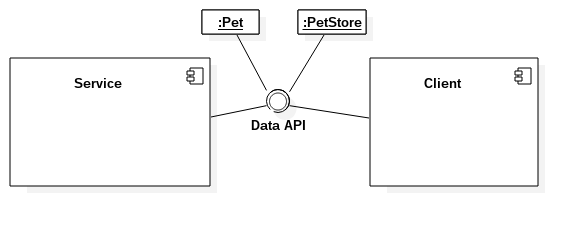
\includegraphics[scale=0.6]{./assets/UML/component1.png}
            \caption{Représentation avec des objets d'une API et ses ressources}
        \end{figure}

        \paragraph{}
            Un premier éssai de modélisation est donné ci-dessus. La première caractéristique d'une telle
            modélisation est l'impossibilité de voir où les ressources sont sollicitées au sein ̂meme
            du composant. De plus, à mesure que le nombre de ressource augmente,  l'encombrement visuel
            du à la représentation des instances passées rend la représentation difficile.

        \begin{figure}[h]
            \centering
            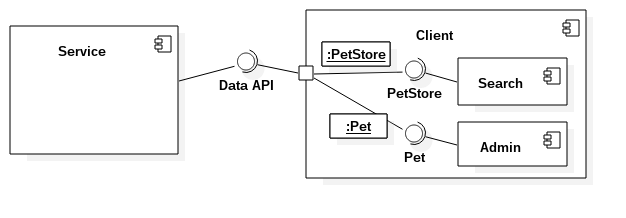
\includegraphics[scale=0.6]{./assets/UML/component3.png}
            \caption{Représentation d'une API et de ses ressources avec des interfaces}
        \end{figure}

        \paragraph{}
            La représentation de l'intéraction avec les sous composants (des WebComponent par exemple)
            est rendue possible par l'utilisation d'interfaces. De plus, pour éviter des diagrammes
            trop verbeux, on proposera la \textbf{convention} suivante pour les diagrammes de composants
            orientés service : \textbf{Une interface est homonyme au ressource qu'elle expose}.

        \begin{figure}[h]
            \centering
            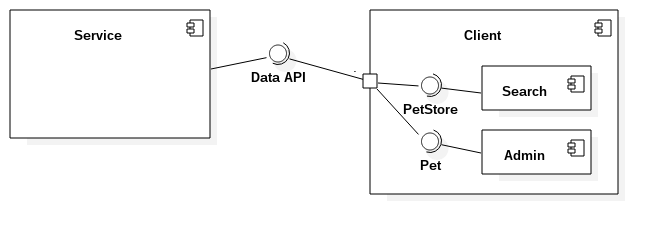
\includegraphics[scale=0.6]{./assets/UML/component2.png}
            \caption{Représentation d'une API et de ses ressources avec des interfaces homonymes aux instances}
        \end{figure}

        \paragraph{}
            Cette utilisation des interfaces renvoie directement à la définition (cf \ref{swaggerdef})
            du formalisme de description d'API Swagger. On remarque alors que le diagramme de composant pour
            les architectures orientées services, est aux formalismes de type Swagger ce que les diagrammes
            de classes sont aux commentaires de type Javadoc : une représentation visuelle alternative.

        \paragraph{}
            Il est intéressant de constater qu'il devient aisé d'avoir une vue globale de l'état
            d'utilisation des services (et donc des ressources) par les différentes parties de ou des
            logiciels. Un bénéfice immédiat de cette modélisation est donc de pouvoir anticiper l'impact
            qu'aurait la modification du fonctionnement d'un service, ou de la modification des modèles
            qui lui sont associés.

    \subsubsection{Représentation des modèles}
        La représentation au niveau composant de l'architecture logicelle a été jugée suffisamment
        détaillée pour ne pas descendre d'échelle et proposer des diagrammes de classes.\\
        En revanche, la question de pose de la représentation des différents modèles annotés en tant
        qu'interfaces sur le diagramme de composant. Pour cela, deux représentations possible :
        le diagramme entité / association (en notation UML ou notation de Chen), ou le diagramme de
        classes. Le premier offre une description d'un point de vue théorique, là ou le second se
        soucie des détails d'implémentations (description des tables de jointures, par exemple).
        Dans la mesure ou l'implémentation de la base de donnée n'a pas été prévue pour changer de
        technologie, il a été choisi de décrire cette dernière à l'aide de diagrammes de classes,
        complémentaires aux diagrammes de composants.

    \subsubsection{Description de l'API}
        Parallèlement au diagrammes de composants qui offrent une vue globale et visuelle des services
        (mais pas forcément exhaustive), nous avons du choisir un formalisme de type Swagger pour
        générer une documention dynamique de l'API.\\
        Le problème que nous avons eu avec Swagger est son principe déterministe\cite{determinism}.
        Il n'est pas possible de définir plusieurs blocs de réponses possible pour un même code http.
        Ainsi, nous avons du nous tourner vers une alternative : APIAry et la syntaxe Blueprint..

    \subsubsection{Commentaires et documentation}
        Nous avons vu au travers l'exemple de Nylas N1 qu'il était possible d'intégrer des larges
        portions de texte de documentation, dans l'optique de réunir code et documentation dans les
        même fichiers. Pour buckless, nous avons jugé cette pratique de vouloir réunir documentation
        et code un peu excessive, car parfois peu lisible au niveau du code source.
        C'est pourquoi nous nous sommes limités à des commentaires de types jsDoc simples.

    \subsubsection{Automatisation}
        Au niveau de l'automatisation de la production de la documentation, le duo linter et
        déploiement continu a été retenu. Pour des raisons de workflow incompatible (évoqué en
        \ref{hooks}), l'utilisation des hooks n'a pas été retenue.

\subsection{Application pratique}
    Dans cette partie, nous essaierons de nous appuyer sur des éléments de documentations pratiques
    qui ont été produits pour le projet, afin de présenter certains mécanismes et choix techniques.
    Buckless étant un projet complexe, seul  les points les plus intéressants, ou les mieux représentés
    seront présentés ici.

    \subsubsection{Architecture globale}
        \begin{figure}[h]
            \centering
            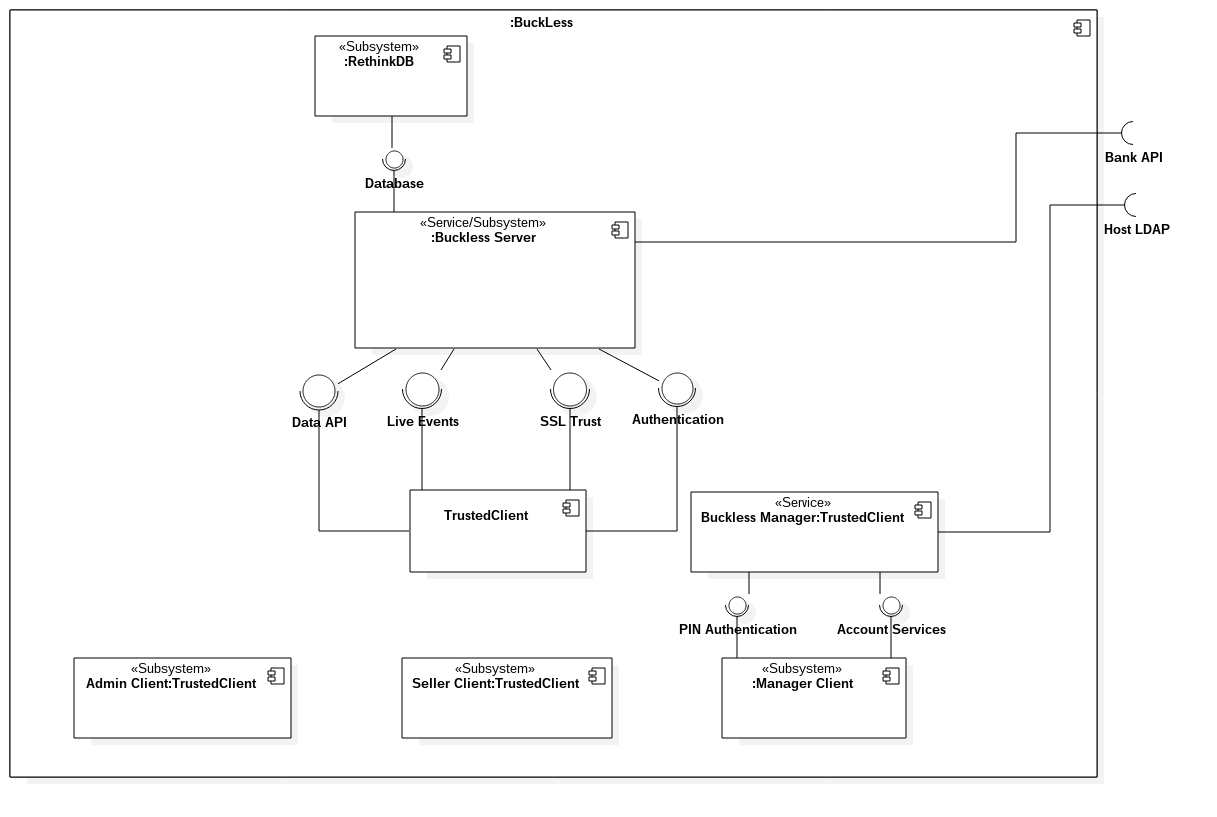
\includegraphics[height=12cm]{./assets/UML/system.png}
        \end{figure}

        \paragraph{}
            Buckless est composé d'une base de données (\textbf{database}) et de quatre grandes briques
            logicielles : une API centrale (\textbf{Buckless Server}), un client de de vente
            (\textbf{Seller client}), un client d'administration (\textbf{Admin client}), et une
            application utilisateur mobile (\textbf{Manager client}).

        \paragraph{}
            Tous les clients de l'API partagent une structure abstraite commune (\textbf{Trusted client}),
            qui consiste en un client disposant des différentes interfaces de l'API sous réserve
            d'une authentification SSL.

        \paragraph{}
            Le système global est dépendant de deux services tiers, l'API de la banque avec laquelle
            les transactions sont faites, et un pentiel annuaire du système d'information hôte
            (le caractère optionnel d'une interface ne peut pas être représenté avec le formalisme du
            diagramme de composant).


    \subsubsection{Architecture serveur}
        \begin{figure}[h]
            \centering
            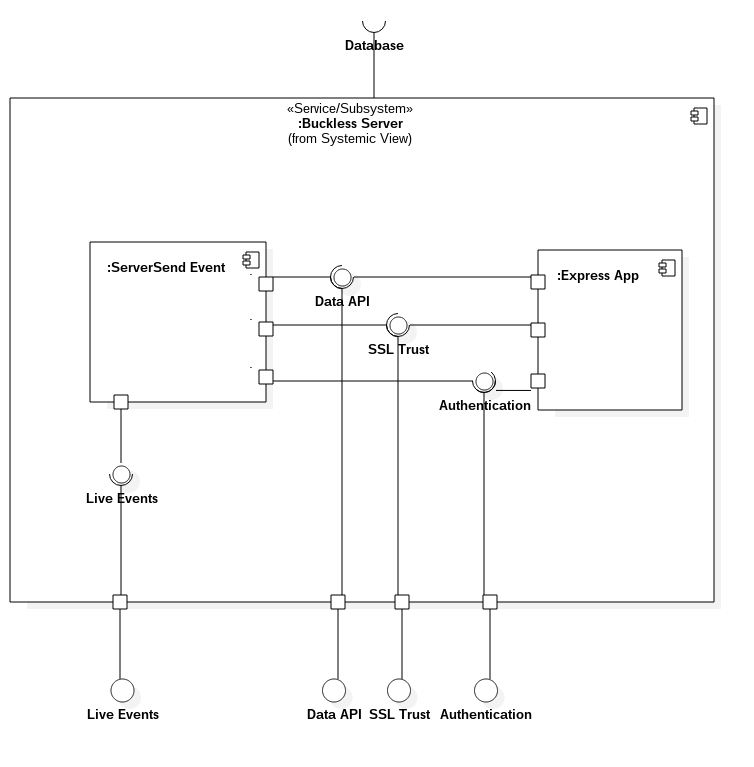
\includegraphics[height=12cm]{./assets/UML/buckless_server.png}
        \end{figure}

        \paragraph{}
            Le serveur a comme unique dépendance la base de donnée. Il est composé d'une API REST
            et d'un composant permettant l'envoi de données depuis le serveur en temps réel.
            L'API REST est développée avec le framework express (\textbf{Express App}). À côté,
            l'envoi des données depuis le serveur vers le client  est fait avec une libraire de Server Send Event (\textbf{SSE}).
            Les deux sont intimement liés, puisque pour récupérer des données, le SSE passe par les différentes méthodes
            exposées par l'application express.

        \paragraph{}
            Les mécanismes de connexion et d'authentification SSL sont faite au travers de \textit{middlewares}
            \footnote{Routines logicielles exécutées entre la connexion et l'applicatif} qui sont encore
            une fois décrits dans une logique commune au deux composants. Ces mises en commun sont représentées
            par des délégation d'interface au sein du composant global \textbf{Buckless Server}.

    \newpage
    \subsubsection{Architecture du client d'administration}
        \begin{figure}[h]
            \centering
            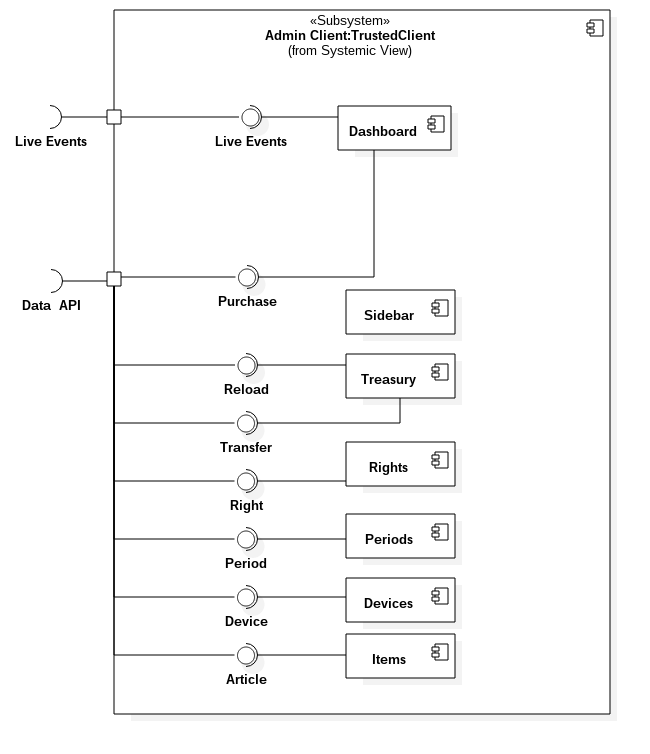
\includegraphics[height=12cm]{./assets/UML/admin_client.png}
        \end{figure}

        Ce diagramme manque cruellement de détail, car cette partie est encore en développement.
        Seule l'idée de base est représentée ici. Chaque sous composant interne représente un WebComponent
        (alliance d'un document html, de son style CSS et de sa logique javascript). L'intérêt ici est
        d'associer chaque WebComponent avec les ressources dont il dépend au niveau de l'API.
        Les dépendances envers l'API REST ainsi que vers les Server Send Events sont représentées par
        des interfaces requises. Au niveau de la \textbf{Data API}, un port est utilisé pour découpler
        l'interface requises en des interfaces fournies. Celles ci respectent la convention de nommage
        des interfaces, qui reflètent les ressources quelles délivrent.

    \newpage
    \subsubsection{Documentation dynamique de l'API}
        \begin{figure}[h]
            \centering
            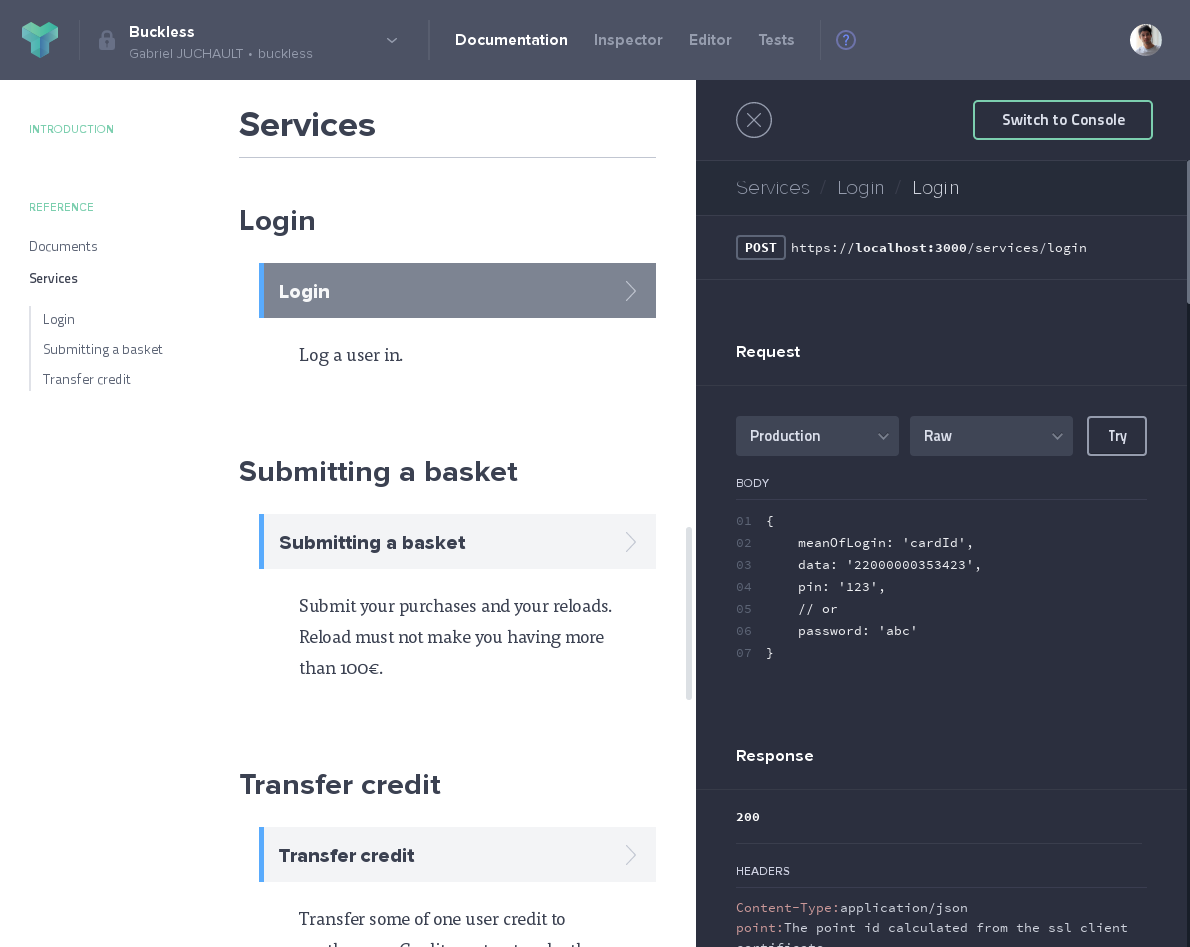
\includegraphics[height=12cm]{./assets/apiary.png}
        \end{figure}
        La documentation dynamique de l'API a été générée par Apiary, un outil semblable à
        celui utilisé par Ghost. Il propose de générer des documentations à partir des plus gros
        formalismes de description d'API (Swagger, API blueprint, RAML).